%!TEX root = ../Thesis.tex
\chapter{Minute-Scale Forecasting of Wind Power}


%--------------------------------------------------------------------------------
\clearpage
\section{Introduction and context}

The International Energy Agency (IEA) was established in the wake of the 1973 oil crisis in order to ensure and regulate security of supply for energy resources in the OECD countries. The wind energy specific sub-programme of the IEA provides a venue for information sharing, research collaboration, and policy review in the form of Research Tasks.

Two relevant Research Tasks were followed as a contributing member during the PhD project.  Task 32 focuses on the maturation and acceptance of wind lidars for various applications in wind energy, including operational control. Task 36 brings together users and creators of wind power forecasts to improve the scientific standards of forecast methods and recommend best practices in the usage of forecast products.

Due to the relevance of both working groups to the PhD project objectives, a goal of merging the two communities for a collaborative workshop was pursued. The workshop was organized alongside fellow researchers in the field Ines W\"urth and Laura Valldecabres Sanmartin, together with the operating agents of Task 36 (Gregor Giebel) and Task 32 (David Schlipf).
The workshop was held at Ris{\o} in June of 2018, and brought together 40 attendees from across the world representing the entire chain of wind energy services.  This includes commercial forecast providers, wind farm operators, research scientists and academics, transmission system operators, wind turbine manufacturers, national meteorological institutes, power trading companies, and lidar manufacturers. 

The workshop was structured with presentations of recent work on the topic, and discussion sessions aimed at collecting inputs from the various perspectives. These included fruitful exchanges on the needs for wind power forecasts on the minute-scale, potential relevant methods to generate them, and possible barriers to adopting them. The workshop presentations were live-streamed and are available in the IEA Task 36 video archive (\cite{iea_36_youtube}).

It was recognized that the recent prominence of the field has led to a distinct gap in knowledge, particularly on a broad level. One of the outcomes of the workshop was the formation of a working group to distill key information into a publicly available document which presents a state of the art review of the field, together with suggestions on future directions to pursue, reached through a consensus approach.

The contributions of the PhD student towards this work include envisioning and co-organizing the workshop and leading discussion groups where the framework and direction of the review paper was decided. Significant writing contributions were made in the sections focusing on intrahour wind variability (Section 2), remote sensing and lidar methods (Sections 5.1 and 5.1.1), statistical time series models (Section 5.2), and the overall comparison of methods (Section 5.5). The portions on data assimilation theory and practices are largely outside the scope of expertise.

The resulting open access journal article is presented in Section \ref{sec:IEA_paper}. 


%--------------------------------------------------------------------------------
\clearpage
\section{Results from the collaborative workshop of IEA Wind Task 32 and 36}
\label{sec:IEA_paper}
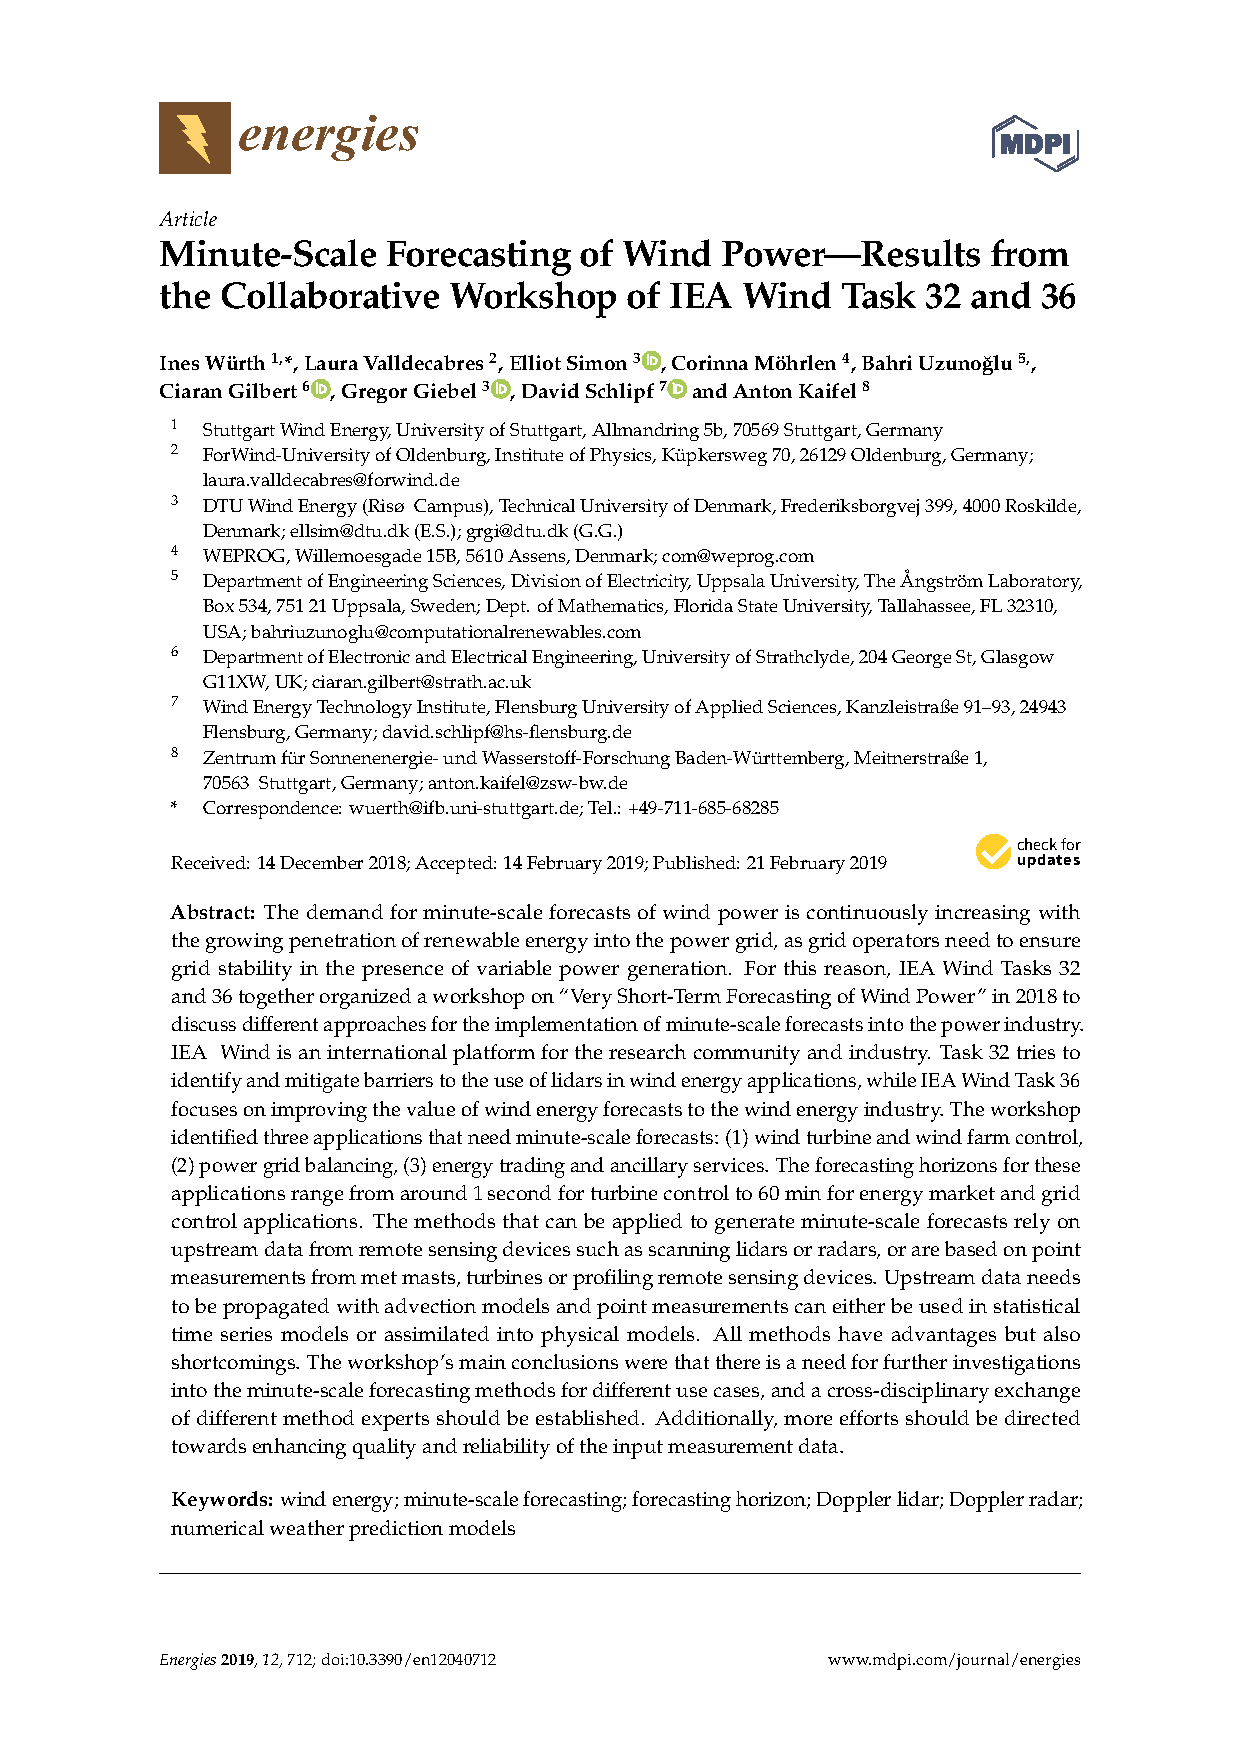
\includepdf[pages=-]{papers/IEA_paper_Energies.pdf}